\documentclass[11pt]{article}
\setlength{\parindent}{0pt}
\usepackage{xltxtra}
\usepackage{hyperref}
\hypersetup{hidelinks}
\usepackage{url}
\urlstyle{tt}
\usepackage{xcolor}
\definecolor{CVBlue}{RGB}{23,110,191}
\usepackage{calc}
\usepackage{graphicx}
\usepackage{tikz}
\usetikzlibrary{calc}
\usepackage{fontspec}
\usepackage{xeCJK}
\usepackage{enumitem}
\CJKsetecglue{} %% 取消中文与数字之间的间隙
%%  主文档字体设置
\setmainfont[
    Path = fonts/Main/,
    Extension = .otf,
    BoldFont = texgyretermes-bold.otf, % 加粗字体
]{texgyretermes-regular.otf} % 正文字体
% 中文字体设置
\setCJKmainfont[
    Path = fonts/hansans/,
    Extension = .ttf,
    BoldFont = NotoSansSC-Bold.ttf, % 加粗字体
]{NotoSansSC-Regular.otf} % 正文字体
\usepackage{relsize}
\usepackage{xspace}
% 使用 fontawesome（部分图标）
\usepackage{fontawesome} 
% A4纸， 上下左右边距
\usepackage[
    a4paper,
    left=1.2cm,
    right=1.2cm,
    top=1.5cm,
    bottom=1cm,
    nohead
]{geometry}
\renewcommand{\baselinestretch}{1.4} % 行间距设为1.5
\usepackage{titlesec}
\usepackage{enumitem}
\setlist{noitemsep} % 取消列表项间的额外间距
%\setlist{nosep} % 取消所有垂直间距
\setlist[itemize]{topsep=0.25em, leftmargin=*}
\setlist[enumerate]{topsep=0.25em, leftmargin=*}
% --- 用于控制【不同项目之间】的垂直距离 ---
\newlength{\interProjectSpacing}
\setlength{\interProjectSpacing}{0.9em} % <--- 在此调整项目之间的距离
\newcommand{\projectsep}{\vspace{\interProjectSpacing}}
% --- 用于控制【项目标题】与下方【项目描述】的距离 ---
\newlength{\intraProjectTitleSep}
\setlength{\intraProjectTitleSep}{0.4em} % <--- 在此调整标题和描述的距离
\newcommand{\titlebreak}{\\[\intraProjectTitleSep]}
% --- 用于控制【项目描述】与下方【要点列表】的距离 ---
\newlength{\intraProjectListTopSep}
\setlength{\intraProjectListTopSep}{0.2em} % <--- 在此调整描述和列表的距离
% =======================================================================
\titleformat{\section}         % 定制 \section 命令 
{\large\bfseries\raggedright} % 将 section 标题设置为大号、粗体且左对齐
{}{0em}                      % 可用于为所有 section 添加前缀（如“章节...”）
{}                           % 可用于在标题前插入代码
[{\color{CVBlue}\titlerule}]  % 在标题后插入一条横线
\titlespacing*{\section}{0cm}{*1.6}{*1.2}
\begin{document}
\pagenumbering{gobble}
%%%% 利用tikz来定位照片
\begin{tikzpicture}[remember picture, overlay] 
    \node[anchor = north east] at ($(current page.north east)+(-2cm,-1.2cm)$) {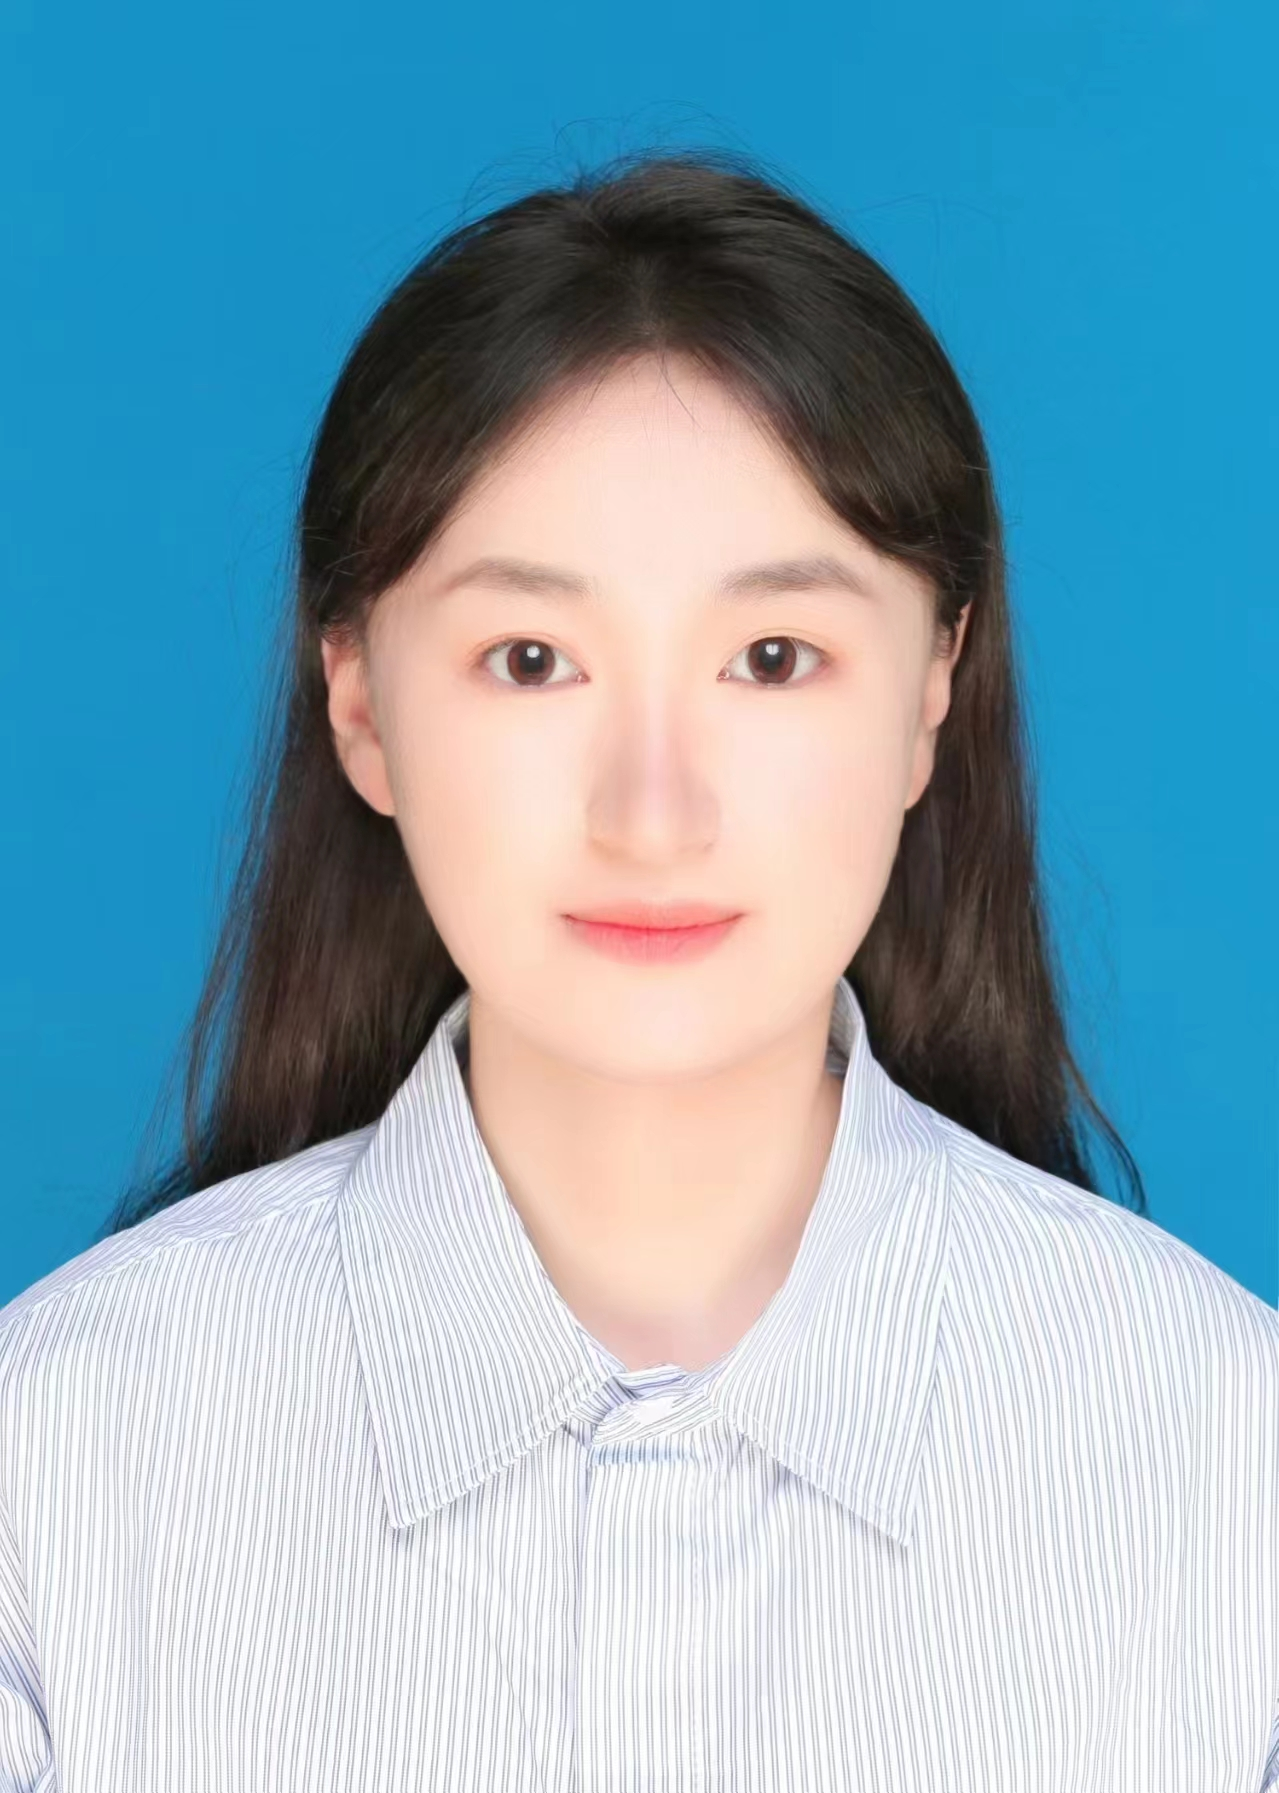
\includegraphics[height=3cm]{avatar.jpg}};
\end{tikzpicture}%
%%%% 利用tikz来定位学校Logo
\begin{tikzpicture}[remember picture, overlay] 
    \node[anchor = north west] at ($(current page.north west)+(1.2cm,-1.2cm)$) {
\includegraphics[height=1.2cm]{hit.jpg}};
\end{tikzpicture}%
% 姓名与联系方式（带定高盒子，完美避开照片并垂直居中）
\vspace*{-0.5em} 
\noindent
\begin{minipage}[c][3cm][c]{\textwidth - 3.5cm}
    \centering
    {\LARGE\bfseries{程昕蕊}}\\[0.4em]
     
    {\large \textbf{AI4Science \textbar 数字孪生 \textbar 大模型算法}}\\[0.5em]
    
    {\normalsize 
        女 $\vert$ 24岁 \quad
        \faPhone\ 150-4336-5908 \quad 
        \faEnvelopeO\ \href{mailto:cxrxin0530@163.com}{cxrxin0530@163.com} \quad
        \faGithubSquare\ \href{https://github.com/chengxinrui/UNOP}{github.com/chengxinrui/UNOP}
        \\\small{政治面貌：\underline{共青团员}}
    }
\end{minipage}
% --- 在这里使用负间距将下方的正文往上拉 ---
\vspace{-0.4cm} 
    
% ================================================================
% 教育背景
% ================================================================
\section{\makebox[\widthof{\faGraduationCap}][c]{\color{CVBlue}\faGraduationCap}\ 教育背景} 
\textbf{哈尔滨工业大学} \quad 软件工程（电子信息） \quad 硕士研究生 \hfill 2024.9 -- 至今\\[0.2em]
\textcolor{CVBlue}{\textbf{排名：前20\%}} \quad \textbf{荣誉：}校级一等、二等学业奖学金；第十五届中兴捧月全球精英挑战赛\textbf{区域优胜奖}

\textbf{长春工业大学} \quad 软件工程 \quad 本科 \hfill 2019.9 -- 2023.6\\[0.2em]
\textcolor{CVBlue}{\textbf{排名：前5\%}} \quad \textbf{荣誉：}校级二等、三等奖学金、单科状元奖学金，累计获奖\textbf{6次}

% ================================================================
% 自我评价
% ================================================================
\section{\makebox[\widthof{\faUser}][c]{\color{CVBlue}\faUser}\ 自我评价}
哈尔滨工业大学软件工程硕士，研究方向为AI4Science、工业数字孪生、物理场智能建模与大模型算法。深度参与“十四五”国家重点研发计划，负责工业三维装备物理场建模算法研发，具备70GB级工业数据处理、AI算法设计、模型规模化部署落地经验；拥有多篇CCF‑A高水平学术论文，多项发明专利与软件著作权。
具备完整的数据治理、模型微调、多维度评测体系搭建工程能力。认同国有能源企业使命，希望运用人工智能与数字孪生技术助力能源行业数字化、智能化转型升级；服从集团岗位调配，意向应聘计算机/人工智能方向管培生岗位。

% ================================================================
% 科研成果概览
% ================================================================
\section{\makebox[\widthof{\faBookmark}][c]{\color{CVBlue}\faBookmark}\ 科研成果概览} 
\textbf{研究聚焦：}面向工业复杂装备开展数字孪生与物理场智能预测研究，研究AI模型在复杂几何条件下的稳定性与泛化能力，推动AI算法向工业真实场景落地。
\begin{itemize}[leftmargin=1.5em]
    \item \textbf{论文成果：}第一作者发表/在投CCF‑A类论文2篇，累计CCF‑A类论文4篇。
    \item \textbf{项目经历：}核心参与\textbf{“十四五”国家重点研发计划}，负责复杂工业三维几何场景下物理场建模与数字孪生算法研发。
    \item \textbf{工程能力：}掌握大规模工业数据处理、AI模型开发部署，实现工业物理场预测推理优化至\textbf{20ms}。
\end{itemize}

% ================================================================
% 国家重点研发项目
% ================================================================
\section{\makebox[\widthof{\faBriefcase}][c]{\color{CVBlue}\faBriefcase}\ 项目经历}
\textbf{复杂工业三维几何下的物理场建模与数字孪生研究}
\textit{\textbf{核心成员，AI算法负责人}}
\hfill 2024.9 -- 2025.6\\[0.2em]
\textcolor{CVBlue}{\textbf{“十四五”国家重点研发计划——装备制造后市场服务协同平台研发与应用}}
\begin{itemize}
    \item 针对工业装备非结构化三维几何拓扑缺陷、尺度异构问题，设计几何拓扑修复与潜空间统一表示框架，完成神经算子算法适配改造。
    \item 在70GB工业三维数据集开展模型验证，实现3D物理场高精度预测，推理时延优化至20ms，完成算法从理论向工业场景迁移。
    \item 独立负责算法架构设计、数据建模策略制定以及核心代码模块实现，产出多项发明专利与软件著作权。
\end{itemize}

% ========================================================
% 学术论文【大幅精简，删除内层嵌套、删除大段痛点创新细节】
% ========================================================
\section{\makebox[\widthof{\faFileTextO}][c]{\color{CVBlue}\faFileTextO}\ 学术论文}
\textbf{第一作者}
\begin{itemize}
    \item Physics‑Constrained Unsupervised Neural Operator for Long‑Horizon PDE Learning on Generalized Geometries，\textbf{IJCAI (CCF‑A)}
    \item Integral‑Consistent Basis‑Universal Neural Operators for Diverse PDE Classes，\textbf{NeurIPS (CCF‑A，在投)}
\end{itemize}

\textbf{共同作者}
\begin{itemize}
    \item Serving Mixture of Experts in Distributed GPU with Route and Graph Execution Selection on Resource‑Constrained Systems，学生一作，\textbf{TPDS (CCF‑A，在投)}，负责MoE分布式推理路径优化。
    \item SeGO: Sensitivity‑Aware Golden Optimization for Large‑Scale VLM Quantization，学生二作，\textbf{IJCAI (CCF‑A)}，负责VLM量化金点搜索算法实现。
    \item Joint Optimization of Fine‑grained Representation and Workflow Orchestration in Metaverse Articulated Manipulation Auto‑generation by VLA Method，五作，\textbf{TSC (CCF‑A)}
    \item MPG‑VLA: Efficient Trajectory Generation for Articulated Objects，三作，\textbf{ICSOC (CCF‑B)}
    \item FD‑MABCVO:A Decentralized, Reliable, Low‑Latency Multi‑base Station Value Chain Collaboration via Human‑UAV Crowdsourcing with Bi‑level Consensus Offloading，四作，\textbf{CCF‑ICSS‑2025}
\end{itemize}

% ================================================================
% 实习经历，末尾增加迁移能力说明
% ================================================================
\section{\makebox[\widthof{\faBuilding}][c]{\color{CVBlue}\faBuilding}\ 实习经历}
\textbf{国科众安科技有限公司} \quad 大模型算法实习生 \hfill 2026.6 -- 2026.9\\[0.2em]
\textcolor{CVBlue}{\textbf{方向：AIGC大模型幻觉治理、文本纠错、检索排序小模型训练与优化}}
\begin{itemize}
    \item \textbf{业务支撑：}面向企业文本校对、知识库检索场景，解决大模型事实幻觉、文本错误、检索精度不足问题。
    \item \textbf{数据工程：}搭建清洗-标注-配比-增强数据流水线，依次完成脏数据自动过滤、人工标注、抽样复核，治理4W+纠错样本、75W+查询-文档对。
    \item \textbf{AIGC幻觉治理与模型微调：}主导中英文文本纠错4B模型LoRA微调，调优样本配比，公开集指标优于原生8B模型；微调Qwen3-Reranker 0.6B，提升知识库检索排序效果。
    \item \textbf{能力迁移：}掌握幻觉治理、数据治理、小模型微调与模型评测全流程，可迁移至能源行业文本、时序、多模态智能业务。
\end{itemize}



% ========================================================
\section{\makebox[\widthof{\faTrophy}][c]{\color{CVBlue}\faTrophy}\ 其他成果}
\begin{itemize}
    \item \textbf{发明专利（实审中）：}一种结合几何特征与傅里叶神经算子的涡轮零件弹性数字孪生虚实交互方法
    \item \textbf{发明专利（实审中）：}基于几何门控注意力机制的结构感知图神经网络物理场预测方法
    \item \textbf{发明专利（已公开）：}一种基于应力驱动转速响应的水轮机风扇智能运维方法
    \item \textbf{软件著作权：}多传感融合的部门数字孪生协同运维平台（登记号：2026SR0202932）
    \item \textbf{软件著作权：}设计‑仿真部门数字孪生协同运维平台（登记号：2026SR0202550）
\end{itemize}

% ================================================================
% 技能与语言【恢复启用，国企必填】
% ================================================================
\section{\makebox[\widthof{\faCogs}][c]{\color{CVBlue}\faCogs}\ 专业技能}
\begin{itemize}
    \item \textbf{编程与框架：}Python、PyTorch、PyG、MS‑SWIFT、Linux、Docker、Git；熟悉深度学习、大模型LoRA微调、神经算子网络开发。
    \item \textbf{工程能力：}大规模工业数据集处理、AI模型训练、调优与部署；具备完整算法评测、对照实验设计能力。
    \item \textbf{外语水平：} 四级、六级，可熟练阅读英文文献，具备英文论文写作投稿经验。
\end{itemize}

\end{document}
